\documentclass[10pt, a4paper, oneside]{ctexart}
\usepackage{minted, multicol, geometry, graphicx, fancyvrb, amssymb}
\usepackage{relsize, setspace, enumitem, float, hyperref, amsmath}
\usepackage[table,xcdraw]{xcolor} % 表格背景颜色
\usepackage{comment} 

\geometry{a4paper, scale = 0.85}

\setenumerate[1]{itemsep=0pt,partopsep=0pt,parsep=\parskip,topsep=0pt}
\setitemize[1]{itemsep=0pt,partopsep=0pt,parsep=\parskip,topsep=0pt}
\setdescription{itemsep=0pt,pa
rtopsep=0pt,parsep=\parskip,topsep=0pt}
\setlength{\parindent}{0pt}
\setlength{\columnsep}{18pt}

\setminted[cpp]{
	style=xcode,
	mathescape,
	linenos,
	autogobble,
	baselinestretch=1,
	tabsize=3,
	fontsize=\scriptsize,
	%bgcolor=Gray,
	frame=single,
	framesep=1mm,
	framerule=0.3pt,
	numbersep=1mm,
	breaklines=true,
	breaksymbolsepleft=2pt,
	%breaksymbolleft=\raisebox{0.8ex}{ \small\reflectbox{\carriagereturn}}, %not moe!
	%breaksymbolright=\small\carriagereturn,
	breakbytoken=false,
	% showtabs=true,
	% tab={\relscale{0.6} $\big\vert \ \ \ $ \relscale{1}},
}

\setminted[bash]{
    style=xcode,
	mathescape,
	linenos,
	autogobble,
	baselinestretch=1,
	tabsize=3,
	fontsize=\scriptsize,
	frame=single,
	framesep=1mm,
	framerule=0.3pt,
	numbersep=1mm,
	breaklines=true,
	breaksymbolsepleft=2pt,
	breakbytoken=false,
}
\setminted[python3]{
    style=xcode,
	mathescape,
	linenos,
	autogobble,
	baselinestretch=1,
	tabsize=3,
	fontsize=\scriptsize,
	frame=single,
	framesep=1mm,
	framerule=0.3pt,
	numbersep=1mm,
	breaklines=true,
	breaksymbolsepleft=2pt,
	breakbytoken=false,
}

\title{ACM 模板}
\author{黄佳瑞,钱智煊,林乐逍}
\date{\today}

\begin{document}
    \scriptsize
    \maketitle
    \newpage
    
    \begin{multicols}{2}
        \tableofcontents
        \newpage

        \section{做题指导}
        \subsection{上机前你应该注意什么}
        \begin{enumerate}
    \item 预估你需要多少机时,以及写出来以后预计要调试多久,并在纸上记下。
    \item 先想好再上机,不要一边写一边想。
    \item 如果有好写的题,务必先写好写的。
    \item 把题目交给擅长的人来写,而不是空闲的人。
\end{enumerate}
        \subsection{机上你应该注意什么}
        \begin{enumerate}
    \item 机时应充分利用,手速应快一些。
    \item 如果你遇到了问题(做法假了、需要分讨等),先下机并通知队友。不要占着机时想。
    \item 建议使用整块时间写题,尽量不要断断续续的写。
\end{enumerate}
        \subsection{交题前你应该注意什么}
        \begin{enumerate}
    \item \verb|long long| 开了没有。
    \item 数组开够没有。
    \item 多测清了没有。
    \item 边界数据 \verb|(corner case)| 考虑了没有
    \item 调试输出删了没有
\end{enumerate}
编译命令:
\inputminted{bash}{src/tools/compile.sh}
        \subsection{如果你的代码挂了}
        按照优先级列出:
\begin{enumerate}
    \item 先 P 再下机。(P 还没有送来就分屏调。)
    \item 看 \verb|long long| 开了没有,数组开够没有,多测清了没有。
    \item 检查 typo ,你有没有打错一些难蚌的地方。
    \item 看看你题读错没有。
    \item 检查你的代码逻辑,即你的代码实现是否与做法一致。同时让另一个人重新读题。
    \item 怀疑做法假了。拉一个人一起看代码。
\end{enumerate}
        \subsection{另外一些注意事项}
        \begin{itemize}
    \item 千万注意节奏,不要让任何一个人在一道题上卡得太久。必要的时候可以换题。
    \item 如果你想要写题,请想好再上机。诸如分类讨论一类的题目,更要想好再上。
    \item 后期的时候可以讨论,没必要一个人挂题。
\end{itemize}

        \newpage
        \section{图论}
        \subsection{Tarjan 边双、点双(圆方树)}
        记录上一个访问的边时要记录边的编号,不能记录上一个过来的节点(因为会有重边)!!!

(如果选择在加边的时候特判,注意编号问题:用输入顺序来对应数组中位置的时候,重边跳过,但是需要 tot+=2。)

圆方树示意图:

\begin{figure}[H]
    \centering
    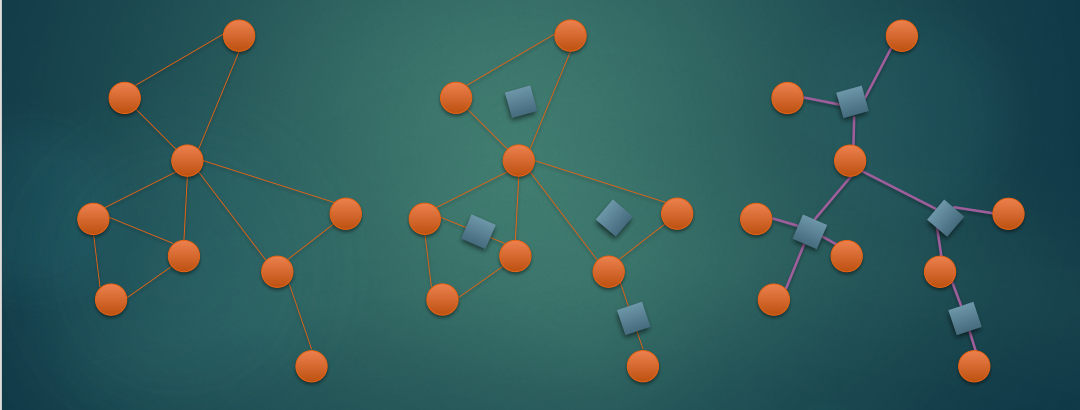
\includegraphics[width=0.45\textwidth]{src/graph/tarjan-tree.png}
    \caption{圆方树示意图}
\end{figure}

\inputminted{cpp}{src/graph/tarjan.cpp}
        \subsection{O(1) LCA}
        按照顺序遍历子树,并查集更新。

\begin{minted}{cpp}
int qhea[Maxq],qver[Maxq],qnex[Maxq],qid[Maxq];
inline void addq(int x,int y,int d)
    { qver[++qtot]=y, qnex[qtot]=qhea[x], qhea[x]=qtot, qid[qtot]=d; }
void dfs(int x,int Last_node)
{
    vis[x]=true;
    for(int i=hea[x];i;i=nex[i])
        if(ver[i]!=Last_node)
            dfs(ver[i],x),fa[ver[i]]=x;
    for(int i=qhea[x];i;i=qnex[i])
        if(vis[qver[i]])
            ans[qid[i]]=Find(qver[i]);
}

for(int i=1;i<=n;i++) fa[i]=i;
for(int i=1,x,y;i<n;i++) x=rd(),y=rd(),add(x,y),add(y,x);
for(int i=1,x,y;i<=m;i++) x=rd(),y=rd(),addq(x,y,i),addq(y,x,i);
dfs(rt,rt);
for(int i=1;i<=m;i++) printf("%d\n",ans[i]);
\end{minted}
        \subsection{2-SAT}
        2-sat 问题定义为:给定 $m$ 个布尔表达式,每个包含两个布尔变量,形如 $a\lor b$ 。求是否存在一种赋值方式,使得所有表达式都为真。

对于表达式 $a\lor b$ ,显然若 $a$ 假则 $b$ 必真,反之亦然。因此,考虑将每个变量拆为两个点,分别代表此变量取值为真或假。对于每个表达式 $a\lor b$ ,连边 $\neg a\to b$ 与 $\neg b\to a$ 。对于边 $u\to v$ ,意义为若 $u$ 为真则 $v$ 必为真。那么对于最后得到的图,如果同一变量拆出的点处在同一强连通分量中,则无解,因为在可行解中它们的取值必然是不同的,但同一强连通分量中的点取值必然相同;否则,考虑缩点以后得到的 DAG ,取其拓扑序,对于每一个变量,令其取拆出的拓扑序较大的点对应的值即可。特别的,以上的判定是必要的,但我还不知道怎么证明它是充分的。
        \subsection{Dinic 网络流、费用流}
        \inputminted{cpp}{src/graph/dinic-flow.cpp}
        \inputminted{cpp}{src/graph/dinic-cost.cpp}
        \subsubsection{无源汇有上下界可行流}
        给定无源汇流量网络 $G$,询问是否存在一种标定每条边流量的方式,使得每条边流量满足上下界同时每一个点流量平衡。

\begin{minted}{cpp}
#include <bits/stdc++.h>
using namespace std;
#define infll 0x3f3f3f3f3f3f3f3f
#define inf 0x3f3f3f3f
#define pb push_back
#define eb emplace_back
#define pa pair<int, int>
#define fi first
#define se second
typedef long long ll;
inline int rd() {
    int x = 0;
    char ch, t = 0;
    while (!isdigit(ch = getchar())) t |= ch == '-';
    while (isdigit(ch)) x = x * 10 + (ch ^ 48), ch = getchar();
    return t ? -x : x;
}
struct Dini {
#define Maxn 505
#define Maxm 20005
    int tot = 1;
    int hea[Maxn], tmphea[Maxn], dep[Maxn];
    int nex[Maxm << 1], ver[Maxm << 1], num[Maxm << 1];
    ll edg[Maxm << 1];
    inline void addedge(int x, int y, int d, int _n) {
        ver[++tot] = y, nex[tot] = hea[x], hea[x] = tot, edg[tot] = d, num[tot] = -1;
        ver[++tot] = x, nex[tot] = hea[y], hea[y] = tot, edg[tot] = 0, num[tot] = _n;
    }
    inline bool bfs(int s, int t) {
        memcpy(tmphea, hea, sizeof(hea));
        memset(dep, 0, sizeof(dep)), dep[s] = 1;
        queue<int> q;
        q.push(s);
        while (!q.empty()) {
            int cur = q.front();
            q.pop();
            if (cur == t) return true;
            for (int i = hea[cur]; i; i = nex[i])
                if (edg[i] > 0 && !dep[ver[i]])
                    dep[ver[i]] = dep[cur] + 1, q.push(ver[i]);
        }
        return false;
    }
    ll dfs(int x, int t, ll flow) {
        if (!flow || x == t) return flow;
        ll rest = flow, tmp;
        for (int i = tmphea[x]; i && rest; i = nex[i]) {
            tmphea[x] = i;
            if (dep[ver[i]] == dep[x] + 1 && edg[i] > 0) {
                if (!(tmp = dfs(ver[i], t, min(rest, edg[i])))) dep[ver[i]] = 0;
                edg[i] -= tmp, edg[i ^ 1] += tmp, rest -= tmp;
            }
        }
        return flow - rest;
    }
    inline ll solve(int s, int t) {
        ll sum = 0;
        while (bfs(s, t))
            sum += dfs(s, t, infll);
        return sum;
    }
#undef Maxn
#undef Maxm
} G;
#define Maxn 205
#define Maxm 10205
int n, m, ss, tt;
int ans[Maxm];
ll needin, needout;
ll Ind[Maxn], Outd[Maxn];
int main() {
    n = rd(), m = rd(), ss = n + 1, tt = n + 2;
    for (int i = 1, x, y, Inf, Sup; i <= m; i++) {
        x = rd(), y = rd(), Inf = rd(), Sup = rd();
        G.addedge(x, y, Sup - Inf, i);
        Outd[x] += Inf;
        Ind[y] += Inf;
        ans[i] = Inf;
    }
    for (int i = 1; i <= n; i++) {
        if (Ind[i] > Outd[i])
            G.addedge(ss, i, Ind[i] - Outd[i], -1), needin += Ind[i] - Outd[i];
        if (Ind[i] < Outd[i])
            G.addedge(i, tt, Outd[i] - Ind[i], -1), needout += Outd[i] - Ind[i];
    }
    ll tmp = G.solve(ss, tt);
    if (needin != needout || needin != tmp) printf("NO\n");
    else {
        for (int i = 2; i <= G.tot; i++)
            if (G.num[i] != -1) ans[G.num[i]] += G.edg[i];
        printf("YES\n");
        for (int i = 1; i <= m; i++) printf("%d\n", ans[i]);
    }
    return 0;
}
\end{minted}
        \subsubsection{有源汇有上下界最大流}
        给定有源汇流量网络 $G$,询问是否存在一种标定每条边流量的方式,使得每条边流量满足上下界同时除了源点和汇点每一个点流量平衡。

假设源点为 $S$,汇点为 $T$,则我们可以加入一条 $T$ 到 $S$ 的上界为 \infty,下界为 $0$ 的边转化为无源汇上下界可行流问题。

若有解,则 $S$ 到 $T$ 的可行流流量等于 $T$ 到 $S$ 的附加边的流量。

\begin{minted}{cpp}
#include <bits/stdc++.h>
using namespace std;
#define infll 0x3f3f3f3f3f3f3f3f
#define inf 0x3f3f3f3f
#define pb push_back
#define eb emplace_back
#define pa pair<int, int>
#define fi first
#define se second
typedef long long ll;
inline int rd() {
    int x = 0;
    char ch, t = 0;
    while (!isdigit(ch = getchar())) t |= ch == '-';
    while (isdigit(ch)) x = x * 10 + (ch ^ 48), ch = getchar();
    return t ? -x : x;
}
struct Dinic {
#define Maxn 505
#define Maxm 20005
    int tot = 1;
    int hea[Maxn], tmphea[Maxn], dep[Maxn];
    int nex[Maxm << 1], ver[Maxm << 1], num[Maxm << 1];
    ll edg[Maxm << 1];
    inline int addedge(int x, int y, ll d, int _n) {
        ver[++tot] = y, nex[tot] = hea[x], hea[x] = tot, edg[tot] = d, num[tot] = -1;
        ver[++tot] = x, nex[tot] = hea[y], hea[y] = tot, edg[tot] = 0, num[tot] = _n;
        return tot;
    }
    inline bool bfs(int s, int t) {
        memcpy(tmphea, hea, sizeof(hea));
        memset(dep, 0, sizeof(dep)), dep[s] = 1;
        queue<int> q;
        q.push(s);
        while (!q.empty()) {
            int cur = q.front();
            q.pop();
            if (cur == t) return true;
            for (int i = hea[cur]; i; i = nex[i])
                if (edg[i] > 0 && !dep[ver[i]])
                    dep[ver[i]] = dep[cur] + 1, q.push(ver[i]);
        }
        return false;
    }
    ll dfs(int x, int t, ll flow) {
        if (!flow || x == t) return flow;
        ll rest = flow, tmp;
        for (int i = tmphea[x]; i && rest; i = nex[i]) {
            tmphea[x] = i;
            if (dep[ver[i]] == dep[x] + 1 && edg[i] > 0) {
                if (!(tmp = dfs(ver[i], t, min(rest, edg[i]))))
                    dep[ver[i]] = 0;
                edg[i] -= tmp, edg[i ^ 1] += tmp, rest -= tmp;
            }
        }
        return flow - rest;
    }
    inline ll solve(int s, int t) {
        ll sum = 0;
        while (bfs(s, t))
            sum += dfs(s, t, infll);
        return sum;
    }
#undef Maxn
#undef Maxm
} G;
#define Maxn 505
#define Maxm 20005
int n, m, ss, tt, s, t;
int ans[Maxm];
ll needin, needout;
ll Ind[Maxn], Outd[Maxn];
int main() {
    n = rd(), m = rd(), s = rd(), t = rd(), ss = n + 1, tt = n + 2;
    for (int i = 1, x, y, Inf, Sup; i <= m; i++) {
        x = rd(), y = rd(), Inf = rd(), Sup = rd();
        G.addedge(x, y, Sup - Inf, i);
        Outd[x] += Inf;
        Ind[y] += Inf;
        ans[i] = Inf;
    }
    for (int i = 1; i <= n; i++) {
        if (Ind[i] > Outd[i])
            G.addedge(ss, i, Ind[i] - Outd[i], -1), needin += Ind[i] - Outd[i];
        if (Ind[i] < Outd[i])
            G.addedge(i, tt, Outd[i] - Ind[i], -1), needout += Outd[i] - Ind[i];
    }
    G.addedge(t, s, infll, -1);
    ll tmp = G.solve(ss, tt);
    if (needin != needout || needin != tmp) printf("please go home to sleep\n");
    else {
        tmp = G.edg[G.tot];
        G.edg[G.tot] = G.edg[G.tot - 1] = 0;
        tmp += G.solve(s, t);
        printf("%lld\n", tmp);
    }
    return 0;
}
\end{minted}
        \subsubsection{网络流总结}
        \subsubsection*{最小割集, 最小割必须边以及可行边}

\paragraph{最小割集} 从 $S$ 出发, 在残余网络中BFS所有权值非 $0$ 的边(包括反向边),得到点集$\{S\}$, 另一集为$\{V\} - \{S\}$. 
\paragraph{最小割集必须点} 残余网络中S直接连向的点必在S的割集中, 直接连向T的点必在T的割集中; 若这些点的并集为全集, 则最小割方案唯一.
\paragraph{最小割可行边} 在残余网络中求强联通分量, 将强联通分量缩点后, 剩余的边即为最小割可行边, 同时这些边也必然满流.
\paragraph{最小割必须边} 在残余网络中求强联通分量, 若S出发可到u, T出发可到v, 等价于$\mathrm{scc}_S=\mathrm{scc}_u$且$\mathrm{scc}_T = \mathrm{scc}_v$, 则该边为必须边.

\subsubsection*{常见问题}

\paragraph{最大权闭合子图}
点权, 限制条件形如: 选择A则必须选择B, 选择B则必须选择C, D. 建图方式: B向A连边, CD向B连边.
求解: S向正权点连边, 负权点向T连边, 其余边容量 $\infty$, 求最小割, 答案为S所在最小割集.
\paragraph{二次布尔型(文理分科)}
$n$ 个点分为两类, $i$ 号点有 $l_{i}$ 或 $r_{i}$ 的代价, $i, j$ 同属一侧分别获得 $l_{ij}$ 或 $r_{ij}$ 的代价, 问最小代价.
$L\rightarrow i: (l_i + 1/2 \sum_{j} l_{ij})$, $i \rightarrow R: (r_i + 1/2 \sum_{j} r_{ij})$,
$i \leftrightarrow j: 1/2 (l_{ij} + r_{ij})$. 实现时边权乘 2 为整数, 求解后答案除 2 为整数. 图拆点可以看作二分图.

如果是二元限制是分类不同时有一个代价 $d_{ij}$,建图可以简化为 $L\rightarrow i: l_i$, $i \rightarrow R: r_i$,
$i \leftrightarrow j: d_{ij}$. 经典例子: \texttt{xor} 最小值, 按位拆开建图.

\paragraph{混合图欧拉回路}把无向边随便定向, 计算每个点的入度和出度, 如果有某个点出入度之差$\mathrm{deg}_i=\mathrm{in}_i-\mathrm{out}_i$为奇数, 肯定不存在欧拉回路. 对于$\mathrm{deg}_i>0$的点, 连接边$(i,T,\mathrm{deg}_i/2)$;对于$\mathrm{deg}_i<0$的点, 连接边$(S,i,-\mathrm{deg}_i/2)$. 最后检查是否满流即可. 
\paragraph{二物流}
水源 $S_1$, 水汇 $T_1$, 油源 $S_2$, 油汇 $T_2$, 每根管道流量共用. 求流量和最大.
建超级源 $SS_1$ 汇 $TT_1$, 连边 $SS_1\to S_1$,$SS_1\to S_2$,$T_1\to TT_1$,$T_2 \to TT_1$, 设最大流为 $x_1$.
建超级源 $SS_2$ 汇 $TT_2$, 连边 $SS_2 \to S_1$, $SS_2\to T_2$,$T_1\to TT_2$, $S_2\to TT_2$, 设最大流为 $x_2$.
则最大流中水流量 $\frac{x_1 + x_2}{2}$, 油流量 $\frac{x_1-x_2}{2}$.

\paragraph{无源汇有上下界可行流}
每条边$(u,v)$ 有一个上界容量$C_{u,v}$和下界容量$B_{u,v}$, 我们让下界变为$0$,上界变为$C_{u,v}-B_{u,v}$, 但这样做流量不守恒. 建立超级源点$SS$和超级汇点$TT$, 用$du_i$来记录每个节点的流量情况, $du_i=\sum B_{j,i}-\sum B_{i,j}$, 添加一些附加弧. 当$du_i>0$时, 连边$(SS,i,du_i)$;当$du_i<0$时, 连边$(i,TT,-du_i)$. 最后对$(SS,TT)$求一次最大流即可, 当所有附加边全部满流时(即$\mathrm{maxflow}==所有du_i>0之和$)时有可行解. 
\paragraph{有源汇有上下界最大可行流}
建立超级源点$SS$和超级汇点$TT$, 首先判断是否存在可行流, 用无源汇有上下界可行流的方法判断. 增设一条从$T$到$S$没有下界容量为无穷的边, 那么原图就变成了一个无源汇有上下界可行流问题. 同样地建图后, 对$(SS,TT)$进行一次最大流, 判断是否有可行解. 
如果有可行解, 删除超级源点$SS$和超级汇点$TT$, 并删去$T$ 到$S$的这条边, 再对$(S,T)$进行一次最大流, 此时得到的$\mathrm{maxflow}$即为有源汇有上下界最大可行流. 
\paragraph{有源汇有上下界最小可行流}
建立超级源点$SS$和超级汇点$TT$, 和无源汇有上下界可行流一样新增一些边, 然后从SS到TT跑最大流. 接着加上边$(T,S,\infty)$, 再从$SS$到$TT$跑一遍最大流. 
如果所有新增边都是满的, 则存在可行流, 此时$T$到$S$这条边的流量即为最小可行流. 
\paragraph{有上下界费用流}
如果求无源汇有上下界最小费用可行流或有源汇有上下界最小费用最大可行流, 用1.6.3.1/1.6.3.2 的构图方法, 给边加上费用即可. 
求有源汇有上下界最小费用最小可行流, 要先用1.6.3.3的方法建图, 先求出一个保证必要边满流情况下的最小费用. 如果费用全部非负, 那么这时的费用就是答案. 如果费用有负数, 那么流多了可能更好, 继续做从$S$到$T$的流量任意的最小费用流, 加上原来的费用就是答案. 
\paragraph{费用流消负环}
新建超级源SS汇TT, 对于所有流量非空的负权边e, 先流满(\texttt{ans+=e.f*e.c, e.rev.f+=e.f, e.f=0}), 再连边SS$\to$e.to, e.from$\to$TT, 流量均为e.f(>0), 费用均为0. 再连边T$\to$S流量$\infty$费用0. 此时没有负环了. 做一遍SS到TT的最小费用最大流, 将费用累加ans, 拆掉T$\to$S的那条边 (此边的流量为残量网络中S$\to$T的流量). 此时负环已消, 再继续跑最小费用最大流.
\begin{comment}
\subsubsection*{二分图最小点覆盖和最大独立集}
\noindent
最小点覆盖: 求出一个最大匹配, 从左部开始每次寻找一个未匹配点, 从该点出发可以得到``未匹配-匹配-未匹配..."形式的交错树, 标记所有这些点. 则最小点覆盖方案为右部未标记点与左部标记点的并集. 显然最小点覆盖集合大小 = 最大匹配.\\
最大独立集 = 全集 - 最小点覆盖.
\end{comment}
\subsubsection*{整数线性规划转费用流}
\noindent
首先将约束关系转化为所有变量下界为$0$, 上界没有要求, 并满足一些等式,
每个变量在均在等式左边且出现恰好两次, 系数为$+1$和$-1$, 优化目标为$\max\sum v_ix_i$的形式.
将等式看做点, 等式i右边的值$b_i$若为正, 则$S$向$i$连边$(b_i, 0)$, 否则i向T连边$(-b_i, 0)$.
将变量看做边, 记变量$x_i$的上界为$m_i$(无上界则$m_i=inf$), 将$x_i$系数为$+1$的那个等式$u$向系数为$-1$的等式$v$连边$(m_i, v_i)$. % 从 nemesis 复制过来的,需要修改
        \subsection{差分约束}
        \textbf{差分约束系统} 是一种特殊的 $n$ 元一次不等式组 。

差分约束系统中的每个约束条件 $x_i-x_j\le c_k$ 都可以变形成 $x_i\le x_j+c_k$ 与 $x_j\ge x_i-c_k$ ,这与单源最短路中的三角形不等式非常相似。因此,我们可以把每个变量 $x_i$ 看做图中的一个结点,对于每个约束条件连边。

需要注意的是,有些题目看能会对解的上、下界进行约束,因此我们需要对这些条件处理(这里只考虑对于这 $n$ 个元素 \textbf{只约束了上界} 或 \textbf{只约束了下界} ):

\begin{itemize}
    \item 只约束下界:有 $0$ 号点向每一个点连一条长为 $Lim_i$ 的边,表示第 $i$ 号元素的 \textbf{下界} 为 $Lim_i$ ,如图所示建边:
    \begin{center}
        \begin{tabular}{|c|c|c|}
            \hline
            题意 & 转化 & 连边 \\
            \hline
            $x_a-x_b\ge c$ & $x_a\ge x_b+c$ & \texttt{add(b,a,c)} \\
            $x_a-x_b\le c$ & $x_b\ge x_a-c$ & \texttt{add(a,b,-c)} \\
            $x_a=x_b$ & $x_a\ge x_b$ , $x_b\le x_a$ & \texttt{add(a,b,0),add(b,a,0)} \\
            \hline
        \end{tabular}
    \end{center}
    之后对整张图跑 \textbf{最长路} 。
    \item 只约束上界:有 $0$ 号点向每一个点连一条长为 $Lim_i$ 的边,表示第 $i$ 号元素的 \textbf{上界} 为 $Lim_i$ ,如图所示建边:
    \begin{center}
        \begin{tabular}{|c|c|c|}
            \hline
            题意 & 转化 & 连边 \\
            \hline
            $x_a-x_b\ge c$ & $x_b\le x_a-c$ & \texttt{add(a,b,-c)} \\
            $x_a-x_b\le c$ & $x_a\le x_b+c$ & \texttt{add(b,a,c)} \\
            $x_a=x_b$ & $x_a\le x_b$ , $x_b\le x_a$ & \texttt{add(a,b,0),add(b,a,0)} \\
            \hline
        \end{tabular}
    \end{center}
    之后对整张图跑 \textbf{最短路} 。
\end{itemize}

设 $dist[0]=0$ ,若存在负环 $/$ 正环,则不等式无解,否则 $x_i=dist[i]$ 是该差分约束系统的一组解 。

最坏情况下(存在负环 $/$ 正环)复杂度为 $O(nm)$ 。

\textbf{注意:整个图不一定是联通的!} 
        \subsection{欧拉路径}
        欧拉图的判定:考虑起点、终点与中间点的必要条件即可。可以证明必要条件也是充分的。
以下给出已确定起点的无向图欧拉路径(回路)的构造算法。
\inputminted{cpp}{src/graph/euler-path.cpp}
        \subsection{同余最短路}
        形如:
\begin{itemize}
    \item 设问 $1$ :给定 $n$ 个整数,求这 $n$ 个整数在 $h(h\le2^{63}-1)$ 范围内 \textbf{能拼凑出多少的其他整数(整数可以重复取)} 。
    \item 设问 $2$ :给定 $n$ 个整数,求这 $n$ 个整数 \textbf{不能拼凑出的最小(最大)的整数} 。
\end{itemize}

设 $x$ 为 $n$ 个数中最小的一个,令 $ds[i]$ 为只通过增加其他 $n-1$ 种数能够达到的最低楼层 $p$ ,并且满足 $p\equiv i\pmod{x}$ 。

对于 $n-1$ 个数与 $x$ 个 $ds[i]$ ,可以如下连边:

\begin{minted}{cpp}
for(int i=0;i<x;i++) for(int j=2;j<=n;j++) add(i,(i+a[j])%x,a[j]);
\end{minted}

之后进行最短路 ,对于 :
\begin{itemize}
    \item 问在 $h$ 范围内能够到达的\textbf{点的数量}:答案为(加一因为 $i$ 本身也要计算)
    \[
    \sum_{i=0}^{x-1}{[d[i]\le h]\times\dfrac{h-d[i]}{x}+1}
    \]
    \item 问不能达到的\textbf{最小的数}:答案为:( $i$ 一定时最小表示的数为 $d[i]=s\times x+i$ ,则 $(s-1)\times x+i$  \textbf{一定不能} 被表示出来 )
    \[
    \min_{i=1}^{x-1}{\{d[i]-x\}}
    \]
\end{itemize}

\textbf{注意:$ds$ 与 $h$ 范围相同,一般也要开 $\operatorname{long}~\operatorname{long}$ !}
        % \subsection{斯坦纳树}
        % \subsubsection{最小割树}

        \section{数据结构}
        \subsection{平衡树}
        \subsubsection{FHQ Treap}
        \inputminted{cpp}{src/data structure/fhq.cpp}
        \subsubsection{平衡树合并}
        如果需要合并两个有交集的 Treap 时该怎么做?我们可以每次将较小的数合并到较大的树中去,这样每个点最多只会合并 $\log n$ 次,每次合并复杂度 $O(n\log n)$,总时间复杂度 $O(n\log n\log V)$。

代码其实非常暴力,就是直接对更小的那棵树直接一个个插入进去:

\inputminted{cpp}{src/data structure/treap-merge.cpp}

\href{https://codeforces.com/blog/entry/108601}{可以证明},若只支持合并与分裂操作,则时间复杂度为 $O(n\log n)$ 。
        \subsubsection{Splay}
        \inputminted{cpp}{src/data structure/splay.cpp} % 没有修改过
        \subsection{LCT 动态树}
        \inputminted{cpp}{src/data structure/LCT.cpp} % EricQian:我不会
        \subsection{ODT 珂朵莉树}
        \inputminted{cpp}{src/data structure/ODT.cpp}
        \subsection{李超线段树}
        \begin{minted}{cpp}
struct Line { double b,k; }a[Maxn];
inline double calc(int p,int x){ return a[p].b+a[p].k*1.0*x; }
inline int tomax(int p1,int p2,int x)
    { return (calc(p1,x)>calc(p2,x)+eps)?p1:p2; }
struct Segment_Tree
{
    int tree[Maxn<<2];
    void add(int p,int nl,int nr,int l,int r,int x)
    {
        int mid=(nl+nr)>>1;
        if(nl>=l && nr<=r)
        {
            if(calc(x,mid)>calc(tree[p],mid)+eps) swap(tree[p],x);
            if(calc(x,nl)>calc(tree[p],nl)+eps) add(p<<1,nl,mid,l,r,x);
            if(calc(x,nr)>calc(tree[p],nr)+eps) add(p<<1|1,mid+1,nr,l,r,x);
            return;
        } // 插入 O(log^2n) :定位到 O(logn) 个区间,每个区间 O(logn) 递归到叶子。
        if(mid>=l) add(p<<1,nl,mid,l,r,x);
        if(mid<r) add(p<<1|1,mid+1,nr,l,r,x);
    }
    int query(int p,int nl,int nr,int x)
    {
        if(nl==nr) return tree[p];
        int mid=(nl+nr)>>1;
        if(mid>=x) return tomax(tree[p],query(p<<1,nl,mid,x),x);
        else return tomax(tree[p],query(p<<1|1,mid+1,nr,x),x);
    }
}T;
\end{minted}

李超线段树的合并本质上和线段树没什么区别,只是在 merge 完两棵子树后的 update 中改为将 $y$ 的最优线段再放到 $x$ 中进行一次 add 即可。

\begin{minted}{cpp}
int merge(int x,int y,int nl,int nr)
{
    if(!x || !y) return x+y;
    int mid=(nl+nr)>>1;
    tree[x].pl=merge(tree[x].pl,tree[y].pl,nl,mid);
    tree[x].pr=merge(tree[x].pr,tree[y].pr,mid+1,nr);
    add(x,nl,nr,tree[y].num);
    return x;
}
\end{minted}
        \subsection{二维树状数组}
        \inputminted{cpp}{src/data structure/2D-BIT.cpp}
        \subsection{虚树}
        \inputminted{cpp}{src/data structure/virtual-tree.cpp}
        \subsection{左偏树}
        \inputminted{cpp}{src/data structure/heap.cpp}
特别的,若要求给定节点所在左偏树的根,须使用并查集。对于每个节点维护 rt[] 值,查找根时使用函数:
\begin{minted}{cpp}
int find(int x) { return rt[x] == x ? x : rt[x] = find(rt[x]); }
\end{minted}
在合并节点时,加入:
\begin{minted}{cpp}
rt[x] = rt[y] = merge(x, y);
\end{minted}
在弹出最小值时加入:
\begin{minted}{cpp}
rt[ls(x)] = rt[rs(x)] = rt[x] = merge(ls(x), rs(x));
\end{minted}
另外,删除过的点是不能复用的,因为这些点可能作为并查集的中转节点。
        \subsection{吉司机线段树}
        \begin{itemize}
    \item 区间取 min 操作:通过维护区间次小值实现,即将区间取 min 转化为对区间最大值的加法,当要取 min 的值 v 大于次小值时停止递归。时间复杂度通过标记回收证明,即将区间最值视作标记,这样每次多余的递归等价于标记回收,总时间复杂度为 $O(m\log n)$。
    \item 区间历史最大值:通过维护加法标记的历史最大值实现。
\end{itemize}
\inputminted{cpp}{src/data structure/seg-beats.cpp}
        \subsection{树分治}
        熟知序列分治的过程是选取恰当的分治点并考虑所有跨过分治点的区间。而树分治的过程也是类似的,以点分治为例,每一次选择当前联通块的重心作为分治点,然后考虑所有跨越分治点的路径,并对分割出的联通块递归。

若要处理树上邻域问题,可以考虑建出点分树。处理点 x 的询问时,只需考虑 x 在点分树上到根的路径,每一次加上除开 x 所在子树的答案即可。

\inputminted{cpp}{src/data structure/tree-divide.cpp}
        % 关于扫描线。
        % 线段树优化建图没有必要。
        % 线段树分治没有必要。
        % 莫队的奇偶优化(看情况)
        % 笛卡尔树计数(为什么要写这种东西)
        % 树分块。
        % 树状数组上二分。
        % ETT 。
        % cdq 以及其它分治。
        % 莫队。

        % exchange argument 。
        
        \section{字符串}
        \subsection{Hash 类}
        \inputminted{cpp}{src/string/hash.cpp}
        \subsection{后缀数组(llx)}
        \inputminted{cpp}{src/string/llx_SA.cpp}
        \subsection{后缀数组与后缀树(旧)}
        \inputminted{cpp}{src/string/SA.cpp}
        \subsection{AC自动机}
        \inputminted{cpp}{src/string/ACAM.cpp}
        \subsection{回文自动机}
        \inputminted{cpp}{src/string/PAM.cpp}
        \subsection{Manacher算法}
        \inputminted{cpp}{src/string/manacher.cpp}
        \subsection{KMP算法与border理论}
        \inputminted{cpp}{src/string/kmp.cpp}
字符串的border理论:
以下记字符串 $S$ 的长度为 $n$ 。
\begin{itemize}
    \item 若串 $S$ 具备长度为 $m$ 的 border ,则其必然具备长度为 $n-m$ 的周期,反之亦然。
    \item 弱周期性引理:若串 $S$ 存在周期 $p$ 、$q$ ,且 $p+q\le n$ ,则 $S$ 必然存在周期 $\gcd(p,q)$ 。
    \item 引理1:若串 $S$ 存在长度为 $m$ 的 border $T$,且 $T$ 具备周期 $p$ ,满足 $2m-n\ge p$ ,则 $S$ 同样具备周期 $p$ 。
    \item 周期性引理:若串 $S$ 存在周期 $p$ 、$q$ ,满足 $p+q-\gcd(p,q)\le n$ ,则串 $S$ 必然存在周期 $\gcd(p,q)$ 。
    \item 引理2:串 $S$ 的所有 border 的长度构成了 $O(\log n)$ 个不交的等差数列。更具体的,记串 $S$ 的最小周期为 $p$ ,则其所有长度包含于区间 $[n \bmod p + p, n)$ 的 border 构成了一个等差数列。
    \item 引理3:若存在串 $S$ 、$T$ ,使得 $2|T|\ge n$ ,则 $T$ 在 $S$ 中的所有匹配位置构成了一个等差数列。
    \item 引理4:PAM 的失配链可以被划分为 $O(\log n)$ 个等差数列。
\end{itemize}
        \subsection{Z函数}
        Z函数用于求解字符串的每一个后缀与其本身的 lcp 。其思路和 manacher 算法基本一致,都是维护一个扩展过的最右端点和对应的起点,而当前点要么暴力扩展使最右端点右移,要么处在记录的起点和终点间,从而可以利用已有的信息快速转移。
\inputminted{cpp}{src/string/zfunc.cpp}
        \subsection{后缀自动机}
        \inputminted{cpp}{src/string/SAM.cpp}
        \subsection{后缀自动机(map版)}
        \inputminted[highlightlines={3,10,15,18}]{cpp}{src/string/SAM_map.cpp}
        \subsection{最小表示法}
        \inputminted{cpp}{src/string/min_pos.cpp}

        \section{线性代数}
        \subsection{高斯消元}
        \inputminted{cpp}{src/linear/gauss.cpp}
        \subsection{线性基}
        \inputminted{cpp}{src/linear/basis.cpp}
        \subsection{行列式}
        容易证明转置后行列式相等,积的行列式等于行列式的积。但是这样的性质并不对和成立,而每次只能拆一行或一列。

以下是任意模数求行列式的算法:
\inputminted{cpp}{src/linear/det.cpp}
        \subsection{矩阵树定理}
        以下叙述允许重边,不允许自环。

对于无向图 $G$ ,定义度数矩阵 $D$ 为:
$$
    D_{ij} = \deg(i)[i=j]
$$
设 $\#e(i,j)$ 为连接点 $i$ 和 $j$ 的边数,定义邻接矩阵 $A$ 为:
$$
    A_{ij} = \#e(i,j)
$$
显然 $A_{ii}=0$ 。
定义 Laplace 矩阵 $L$ 为 $D-A$ ,记 $G$ 的生成树个数为 $t(G)$ ,则其恰为 $L$ 的任意一个 $n-1$ 阶主子式的值。

对于有向图 $G$ ,分别定义出度矩阵 $D^{out}$ 和入度矩阵 $D^{in}$ 为:
$$
    \begin{aligned}
        D^{out}_{ij} & = \deg^{out}(i)[i=j] \\
        D^{in}_{ij}  & = \deg^{in}(i)[i=j]
    \end{aligned}
$$
设 $\#e(i,j)$ 为从点 $i$ 到 $j$ 的边数,定义邻接矩阵 $A$ 为:
$$
    A_{ij} = \#e(i,j)
$$
显然 $A_{ii}=0$ 。
再分别定义出度 Laplace 矩阵 $L^{out}$ 和入度 Laplace 矩阵 $L^{in}$ 为:
$$
    \begin{aligned}
        L^{out} & = D^{out}-A \\
        L^{in}  & = D^{in}-A
    \end{aligned}
$$
分别记 $G$ 的以 $k$ 为根的根向树形图个数为 $t^{root}(k)$ ,以及以 $k$ 为根的叶向树形图个数为 $t^{leaf}(k)$ 。则 $t^{root}(k)$ 恰为 $L^{out}$ 的删去 $k$ 行 $k$ 列的 $n-1$ 阶主子式的值;$t^{leaf}(k)$ 恰为 $L^{in}$ 的删去 $k$ 行 $k$ 列的 $n-1$ 阶主子式的值。
        \subsection{单纯形法}
        线性规划的标准型:

$$
\begin{aligned}
	{\rm maximize}: & & c^{\rm T}x\\
	{\rm constraints}: & & Ax\le b\\
	& & x\ge 0
\end{aligned}
$$

在标准型的基础上得到松弛型:

$$
\begin{aligned}
    {\rm maximize}: & & c^{\rm T}x\\
    {\rm constraints}: & & \alpha=b-Ax\\
    & & \alpha,x\ge 0
\end{aligned}
$$

单纯性法以松弛型为基础。具体的,松弛型隐含了一个基本解,即 $x=0$ ,$\alpha = b$(这里要求 $b\ge 0$ )。我们称 $\alpha$ 中的变量为基变量,其余为非基变量。单纯性的主过程被称作 pivot 操作。一次 pivot 操作的本质就是进行基变量与非基变量之间的变换以使得带入基本解的目标函数更大。具体的,我们每一次选定一个在目标函数中系数为正的变量为换入变量,再选择对这个换入变量约束最紧的的线性约束所对应的基变量,称其为换出变量。然后,我们将换入变量和换出变量分别换为基变量和非基变量,并对其余的式子做出对应的代换以使得定义满足即可。

另外单纯型法的时间复杂度虽然是指数级别的,但是跑起来效果还是很好的,期望迭代次数貌似可以大致看作约束个数的平方级别。

\inputminted{cpp}{src/linear/simplex.cpp}
        \subsection{全幺模矩阵}
        当一个矩阵的任意一个子方阵的行列式都为 $\pm1,0$ 时,我们称这个矩阵是全幺模的。

如果单纯形矩阵是全幺模的,那么单纯形就具有整数解。
        \subsection{对偶原理}
        线性规划的对偶原理:原线性规划与对偶线性规划的最优解相等。即:
$$
\begin{aligned}
    {\rm minimize}: & & c^{\rm T}x & & & & {\rm maximize}:& & b^{\rm T}y \\
    {\rm constraints}: & & Ax\ge b &  & {\rm dual} & & {\rm constraints}:& & A^{\rm T}y\le c\\
    & & x\ge 0 & & & & & & y\ge 0
\end{aligned}
$$
直观上看,对于一个最小化的线性规划,我们尝试构造一个最大化的线性规划,使得它们目标函数的最优解相同。具体的,为每个约束设置一个非负的新变量,代表其系数。对于每个原变量,其对应了一个新约束,要求原约束的线性组合的对应系数不大于原目标函数的系数,从而得到原目标函数的下界。而新目标函数则要使得原约束的组合最大化,从而得到最紧的下界。而线性规划对偶性则指出,原线性规划的最优解必然与对偶线性规划的最优解相等。

对偶线性规划具备互补松弛性。即,设 $x$ 和 $y$ 分别为原问题与对偶问题的可行解,则 $x$ 和 $y$ 均为最优解,当且仅当以下两个命题同时成立:
$$
    \begin{aligned}
        \forall j\in[1,m], x_j=0\lor\sum_{i=1}^n a_{ij}y_i=c_j\\
        \forall i\in[1,n], y_i=0\lor\sum_{j=1}^m a_{ij}x_j\le b_i\\
    \end{aligned}
$$
对偶松弛性的意义是,其指出若最优解中的变量不取 $0$ ,则对应约束在最优解中一定取等。
        % 记得写格林公式之类的。

        \section{多项式}
        \subsection{FFT}
        \inputminted{cpp}{src/poly/fft.cpp}
        \subsection{NTT}
        \inputminted{cpp}{src/poly/ntt.cpp}
        \subsection{集合幂级数}
        \subsubsection{并卷积、交卷积与子集卷积}
        集合并等价于二进制按位或,因此并卷积的计算实际上就是做高维前缀和以及差分,也被称作莫比乌斯变换。
\inputminted{cpp}{src/poly/or.cpp}
而集合交卷积则对应后缀和。
\inputminted{cpp}{src/poly/and.cpp}
子集卷积则较为特殊,为了使得产生贡献的集合没有交集,考虑引入代表集合大小的占位符。这样只需做 $n$ 次 FMT ,再枚举长度做 $n^2$ 次卷积。因为 FMT 具备线性性,所以最后只需做 $n$ 次 iFMT 即可。
\inputminted{cpp}{src/poly/linear.cpp}
特别的,子集卷积等价于 $n$ 元保留到一次项的线性卷积。
        \subsubsection{对称差卷积}
        集合对称差等价于按位异或,而异或卷积则等价于 $n$ 元模 $2$ 的循环卷积,因此,FWT 实质上和 $n$ 元 FFT 没有什么区别。
\inputminted{cpp}{src/poly/xor.cpp}
        \subsection{多项式全家桶}
        \inputminted{cpp}{src/poly/poly.cpp}

        \section{数论}
        \subsection{中国剩余定理}
        $$
\begin{cases}
	x\equiv a_1 \pmod {m_1}\\
	x\equiv a_2 \pmod {m_2}\\
	\cdots\\
	x\equiv a_n \pmod {m_n}\\
\end{cases}
$$
求解 $x$ ,其中 $m_1,m_2,\dots m_n$ 互素。
$$
x\equiv\sum_{i=1}^na_i\prod_{j\neq i}^n m_j\times\left(\left(\prod_{j\neq i}^n m_j\right)^{-1}\pmod{m_i}\right)\pmod{\prod_{i=1}^n m_i}
$$
        \subsection{扩展中国剩余定理}
        用于求解同余方程组的模数并不互素的情况。我们考虑如何合并两个同余式:
$$
\begin{cases}
	x \equiv a_1 \pmod {m_1}\\
	x \equiv a_2 \pmod {m_2}\\
\end{cases}
$$
显然其等价于:
$$
\begin{cases}
	x = a_1 + k_1\times m_1\\
	x = a_2 + k_2\times m_2\\
\end{cases}
$$
联立可得:
$$
k_1m_1-k_2m_2=a_2-a_1
$$
我们解这个方程即可得出当前的解 $x_0$ 。且注意到我们若给 $x_0$ 加上若干个 $\operatorname{lcm}(m_1,m_2)$ ,上式仍然成立,即当前的解是在 $\bmod \operatorname{lcm}(m_1,m_2)$ 意义下的。这样我们得出新的同余式:
$$
x\equiv x_0 \pmod {\operatorname{lcm}(m_1,m_2)}
$$
与其它式子继续合并即可。注意在数据范围比较大的时候需要龟速加。
        \subsection{BSGS}
        在 $\sqrt{p}$ 的时间内求解 $a^x\equiv b\pmod{p}$,要求 $a$ 与 $p$ 互质。
\inputminted{cpp}{src/number theory/bsgs.cpp}
        \subsection{扩展 BSGS}
        不要求 $a,p$ 互质。
\inputminted{cpp}{src/number theory/exbsgs.cpp}
        \subsection{Lucas 定理}
        \inputminted{cpp}{src/number theory/lucas.cpp}
        \subsection{扩展 Lucas 定理}
        \inputminted{cpp}{src/number theory/exlucas.cpp}
        \subsection{杜教筛}
        实际上是利用迪利克雷卷积来构造递推式,从而对一些积性函数快速求和的方法。

我们现在考虑求取积性函数 $f$ 的前缀和 $F$ 。设存在函数 $g$ ,使得 $f*g$ 的前缀和可以被快速计算,那么:
$$
\begin{aligned}
	\sum_{k=1}^n(f*g)(k)
	&=\sum_{k=1}^n\sum_{d\mid k}f\left(\frac kd\right)\times g(d)\\
	&=\sum_{d=1}^n\sum_{k=1}^{\lfloor n/ d \rfloor} f(k) \times g(d)\\
	&=\sum_{d=1}^ng(d)\times F\left(\left\lfloor\frac nd\right\rfloor\right)\\
	&=\sum_{d=2}^ng(d)\times F\left(\left\lfloor\frac nd\right\rfloor\right)+g(1)\times F(n)\\
\end{aligned}
$$
则:
$$
F(n)=\left(\sum_{k=1}^n(f*g)(k)-\sum_{d=2}^ng(d)\times F\left(\left\lfloor\frac nd\right\rfloor\right)\right){\bigg /} g(1)
$$
若 $f*g$ 的前缀和可以被快速计算,我们就可以使用整除分块,从而把 $F(n)$ 划分为若干个子问题。使用时使用线性筛来预处理 $F$ 的前 $n^{\frac 23}$ 项,这样杜教筛的时间复杂度为 $O(n^{\frac 23})$ 。
        \subsection{Min-25筛}
        Min-25 筛本质上是对埃氏筛进行了扩展,用于求解积性函数的前缀和,要求其在质数与质数的次幂处的取值可以被快速计算。

下面对 Min-25 筛的运行过程做一个简要的推导:

记 $\mathbb P$ 中的数为 $p$ ,$p_k$ 为 $\mathbb P$ 中第 $k$ 小的数,${\rm lpf}(n)$( $\rm lowest\ prime\ factor$ )为 $n$ 的最小素因子,$F(n)=\sum_{p\le n}f(p)$ ,$F_k(n)=\sum_{i=2}^n[p_k\le{\rm lpf}(i)]f(i)$ ,不难发现答案即为 $F_1(n)+1$ 。

考虑在 $F_k$ 与 $F$ 之间建立递推关系,从素因子的角度出发,并应用积性函数的性质,我们有:
$$
\begin{aligned}
	F_k(n)&=\sum_{i=1}^n[{\rm lpf}(i)\ge k]f(i) \\
	&=\sum_{i\ge k,p_i^2\le n}\sum_{c\ge 1,p_i^c\le n} f(p_i^c)\times([c>1]+F_{k+1}(n/p_i^c))+F(n)-F(p_{k-1})\\
\end{aligned}
$$
现在的问题在于如何快速求取 $F$ 。首先可以注意到只有 $O(\sqrt n)$ 处的 $F_k$ 和 $F$ 的取值对我们来说是有用的,这一点保障了我们的计算复杂度。现在我们只关注 $f$ 在质数处的取值,在具体的问题中,这一部分往往可以被表示为一个低次多项式,因此我们可以考虑分别计算每一项的贡献,最后再把它们加起来。也就是说现在我们只需要求 $g(n)=n^s$ 在只考虑素数处的取值的情况下的前缀和。注意到 $g$ 具有非常优美的性质,其是一个完全积性函数,因此我们考虑构造 $G_k(n)=\sum_{i=2}^n[{\rm lpf}(i)>p_k \lor i \in {\mathbb P}]g(i)$ ,即埃氏筛第 $k$ 轮以后剩下的数处的 $g$ 的取值之和。从埃氏筛的过程入手,我们考虑如何递推求解 $G_k(n)$ ,即:

1. 对于 $p_k^2>n$ ,显然,所有满足的条件的数都会是素数,因此 $G_k(n)=G_{k-1}(n)$ 。
2. 否则我们希望去除掉所有 ${\rm lpf}$ 为 $p_k$ 的合数处的取值,即减去 $g(p_k)G_{k-1}(n/p_k)$ 。
3. 在第 $2$ 步中会多减一部分,这部分均仅含一个小于 $p_k$ 的素因子,因此我们加上 $g(p_k)G_{k-1}(p_{k-1})$ 。

概括一下,我们有:
$$
G_k(n)=G_{k-1}(n)-[p_k^2\le n]g(p_k)(G_{k-1}(n/p_k)-G_{k-1}(p_{k-1}))
$$

以下是洛谷 P5325 求积性函数 $f(p^k)=p^k(p^k-1),p\in\mathbb P$ 的前缀和的代码:
\inputminted{cpp}{src/number theory/min25.cpp}

        \section{计算几何}
        \subsection{声明与宏}
        \inputminted{cpp}{src/geometry/define.cpp}
        \subsection{点与向量}
        \inputminted{cpp}{src/geometry/vector.cpp}
        \subsection{线}
        \inputminted{cpp}{src/geometry/line.cpp}
        \subsection{圆}
        \inputminted{cpp}{src/geometry/circle.cpp}
        \subsection{凸包}
        \inputminted{cpp}{src/geometry/convex.cpp}
        \subsection{三角形}
        \inputminted{cpp}{src/geometry/triangle.cpp}
        \subsection{多边形}
        \inputminted{cpp}{src/geometry/polygon.cpp}
        \subsection{半平面交}
        \inputminted{cpp}{src/geometry/half-plane.cpp}

        \section{杂项}
        \subsection{生成树计数}
        【根据度数求方案】对于给定每个点度数为 $d_i$ 的无根树,方案数为:
$$
\dfrac{(n-2)!}{\prod_{i=1}^{n}(d_i-1)!}
$$
【根据连通块数量与大小求方案】一个 $n$ 个点 $m$ 条边的带标号无向图有 $k$ 个连通块,每个连通块大小为 $s_i$,需要增加 $k-1$ 条边使得整个图联通,方案数为:(但是当 $k=1$ 时需要特判)
$$
n^{k-2}\cdot\prod_{i=1}^{k}s_i
$$
证明只需考虑 prufer 序列即可。
        \subsection{类欧几里得}
        $ax+by=n$ 的几何意义可以想象为一条直线,那么 $[0,n]$ 中可以被表示出来的整数就是 $(0,0),\left(\frac{n}{a},0\right),\left(0,\frac{n}{b}\right)$ 为顶点的三角形在第一象限内含有的整点个数。

显然的结论就是,在 $[0,n]$ 可以表示出的整数数量为:
$$
\sum_{x=0}^{\lfloor\frac{n}{a}\rfloor}\left\lfloor\dfrac{n-ax}{b}\right\rfloor
$$
类欧几里得可以在 $\mathcal{O(\log{\max(a,b)})}$ 的时间内解决此类问题。

求 $\sum_{i=0}^{n}\lfloor \frac{ai+b}{c} \rfloor$ :
\inputminted{cpp}{src/else/euclid1.cpp}
求 $\sum_{i=0}^{n}{\lfloor \frac{ai+b}{c} \rfloor}^2$ 和 $\sum\limits_{i=0}^{n}i\lfloor \frac{ai+b}{c} \rfloor$ ,分别对应以下的 \verb|g| 和 \verb|h| :
\inputminted{cpp}{src/else/euclid2.cpp}

        \section{其它工具}
        \subsection{编译命令}
        \inputminted{bash}{src/tools/compile.sh}
        \subsection{快读}
        \inputminted{cpp}{src/tools/fastio.cpp}
        \subsection{Python Hints}
        \inputminted{python3}{src/tools/python_hint.py}
        \subsection{对拍器}
        \inputminted{python3}{src/tools/llx_checker.py}
        \subsection{常数表}
        \begin{table}[H]
\centering
\resizebox{\columnwidth}{!}{
\begin{tabular}{|l|l|l|l|l|}
\hline
\rowcolor[HTML]{C0C0C0} 
$n$ & $\log_{10} n$ & $n!$ & $C(n,n/2)$ & $\operatorname{lcm}(1...n)$ \\
2          & 0.301030   & 2              & 2              & 2              \\\hline
3          & 0.477121   & 6              & 3              & 6              \\\hline
4          & 0.602060   & 24             & 6              & 12             \\\hline
5          & 0.698970   & 120            & 10             & 60             \\\hline
6          & 0.778151   & 720            & 20             & 60             \\\hline
7          & 0.845098   & 5040           & 35             & 420            \\\hline
8          & 0.903090   & 40320          & 70             & 840            \\\hline
9          & 0.954243   & 362880         & 126            & 2520           \\\hline
10         & 1.000000   & 3628800        & 252            & 2520           \\\hline
11         & 1.041393   & 39916800       & 462            & 27720          \\\hline
12         & 1.079181   & 479001600      & 924            & 27720          \\\hline
15         & 1.176091   & 1.31e12        & 6435           & 360360         \\\hline
20         & 1.301030   & 2.43e18        & 184756         & 232792560      \\\hline
25         & 1.397940   & 1.55e25        & 5200300        & 2.68e10        \\\hline
30         & 1.477121   & 2.65e32        & 155117520      & 2.33e12        \\\hline
\end{tabular}
}
\end{table}

\begin{table}[H]
\centering
\resizebox{\columnwidth}{!}{
\begin{tabular}{|l|llllll|}
\hline
\rowcolor[HTML]{C0C0C0} 
$n\le$              & \multicolumn{1}{l|}{\cellcolor[HTML]{C0C0C0}$10^1$}  & \multicolumn{1}{l|}{\cellcolor[HTML]{C0C0C0}$10^2$}  & \multicolumn{1}{l|}{\cellcolor[HTML]{C0C0C0}$10^3$}  & \multicolumn{1}{l|}{\cellcolor[HTML]{C0C0C0}$10^4$}    & \multicolumn{1}{l|}{\cellcolor[HTML]{C0C0C0}$10^5$}  & \cellcolor[HTML]{C0C0C0}$10^6$ \\ \hline
$\max\{\omega(n)\}$ & \multicolumn{1}{l|}{2}                               & \multicolumn{1}{l|}{3}                               & \multicolumn{1}{l|}{4}                               & \multicolumn{1}{l|}{5}                                 & \multicolumn{1}{l|}{26}                              & 7                              \\ \hline
$\max\{d(n)\}$      & \multicolumn{1}{l|}{4}                               & \multicolumn{1}{l|}{12}                              & \multicolumn{1}{l|}{32}                              & \multicolumn{1}{l|}{64}                                & \multicolumn{1}{l|}{128}                             & 240                            \\ \hline
$\pi(n)$            & \multicolumn{1}{l|}{4}                               & \multicolumn{1}{l|}{25}                              & \multicolumn{1}{l|}{168}                             & \multicolumn{1}{l|}{1229}                              & \multicolumn{1}{l|}{9592}                            & 78498                          \\ \hline
\rowcolor[HTML]{C0C0C0} 
$n\le$              & \multicolumn{1}{l|}{\cellcolor[HTML]{C0C0C0}$10^7$}  & \multicolumn{1}{l|}{\cellcolor[HTML]{C0C0C0}$10^8$}  & \multicolumn{1}{l|}{\cellcolor[HTML]{C0C0C0}$10^9$}  & \multicolumn{1}{l|}{\cellcolor[HTML]{C0C0C0}$10^{10}$} & \multicolumn{1}{l|}{\cellcolor[HTML]{C0C0C0}$10^{11}$} & $10^{12}$                        \\ \hline
$\max\{\omega(n)\}$ & \multicolumn{1}{l|}{8}                               & \multicolumn{1}{l|}{8}                               & \multicolumn{1}{l|}{9}                               & \multicolumn{1}{l|}{10}                                & \multicolumn{1}{l|}{10}                              & 11                             \\ \hline
$\max\{d(n)\}$      & \multicolumn{1}{l|}{448}                             & \multicolumn{1}{l|}{768}                             & \multicolumn{1}{l|}{1344}                            & \multicolumn{1}{l|}{2304}                              & \multicolumn{1}{l|}{4032}                            & 6720                           \\ \hline
$\pi(n)$            & \multicolumn{1}{l|}{664579}                          & \multicolumn{1}{l|}{5761455}                         & \multicolumn{1}{l|}{5.08e7}                          & \multicolumn{1}{l|}{4.55e8}                            & \multicolumn{1}{l|}{4.12e9}                          & 3.7e10                         \\ \hline
\rowcolor[HTML]{C0C0C0} 
$n\le$              & \multicolumn{1}{l|}{\cellcolor[HTML]{C0C0C0}$10^{13}$} & \multicolumn{1}{l|}{\cellcolor[HTML]{C0C0C0}$10^{14}$} & \multicolumn{1}{l|}{\cellcolor[HTML]{C0C0C0}$10^{15}$} & \multicolumn{1}{l|}{\cellcolor[HTML]{C0C0C0}$10^{16}$}   & \multicolumn{1}{l|}{\cellcolor[HTML]{C0C0C0}$10^{17}$} & $10^{18}$                        \\ \hline
$\max\{\omega(n)\}$ & \multicolumn{1}{l|}{12}                              & \multicolumn{1}{l|}{12}                              & \multicolumn{1}{l|}{13}                              & \multicolumn{1}{l|}{13}                                & \multicolumn{1}{l|}{14}                              & 15                             \\ \hline
$\max\{d(n)\}$      & \multicolumn{1}{l|}{10752}                           & \multicolumn{1}{l|}{17280}                           & \multicolumn{1}{l|}{26880}                           & \multicolumn{1}{l|}{41472}                             & \multicolumn{1}{l|}{64512}                           & 103680                         \\ \hline
$\pi(n)$            & \multicolumn{6}{l|}{$\pi(x)\sim x/\ln(x)$}                                                                                                                                                                                                                                                                          \\ \hline
\end{tabular}
}
\end{table}
        \subsection{试机赛}
        \begin{itemize}
    \item 测试编译器版本。
    \begin{itemize}
        \item  \texttt{\#include<bits/stdc++.h>}
        \item  \texttt{pb\_ds}
        \item  C++20: \texttt{cin>>(s+1);}
        \item  C++17: \texttt{auto [x,y]=pair{1,"abc"};}
        \item  C++11: \texttt{auto x=1;}
    \end{itemize}
    \item 测试 \_\_int128, \_\_float128, long double
    \item 测试 pragma 是否 CE 。
    \item 测试 ‐fsanitize=address,undefined
    \item 测试本地性能
        % TODO 测试性能代码
\end{itemize}




        % \subsubsection{linux}
        % \inputminted{cpp}{src/tools/linux_checker.cpp}
        % \subsubsection{windows}
        % \inputminted{cpp}{src/tools/win_checker.cpp}
        \subsection{阴间错误集锦}
        \begin{itemize}
    \item 多测不清空。
    \item 该开 \verb|long long| 的地方不开 \verb|long long| 。一般情况下建议直接 \verb|#define int long long| 。
    \item 注意变量名打错。例如 u 打成 v 或 a 打成 t 。建议读代码的时候专门检查此类错误。
\end{itemize}
        % 构建表达式树
    \end{multicols}
\end{document}